%\pdfoutput=0
\documentclass[twocolumn]{article}
\usepackage{graphicx}
\title{An example of using \LaTeX and Gnuplot: the sinusiodal function}
\author{Frederik ~Lillebaek}
\begin{document}
\maketitle
In mathematics, the sine is a trigonometric function of an angle. The sine of an acute angle is defined in the context of a right triangle: for the specified angle, it is the ratio of the length of the side that is opposite that angle to the length of the longest side of the triangle (the hypotenuse).

More generally, the definition of sine (and other trigonometric functions) can be extended to any real value in terms of the length of a certain line segment in a unit circle. More modern definitions express the sine as an infinite series or as the solution of certain differential equations, allowing their extension to arbitrary positive and negative values and even to complex numbers.

The sine function is commonly used to model periodic phenomena such as sound and light waves, the position and velocity of harmonic oscillators, sunlight intensity and day length, and average temperature variations throughout the year.

The function sine can be traced to the jyā and koṭi-jyā functions used in Gupta period Indian astronomy (Aryabhatiya, Surya Siddhanta), via translation from Sanskrit to Arabic and then from Arabic to Latin.[1] The word "sine" (Latin "sinus") comes from a Latin mistranslation by Robert of Chester of the Arabic jiba, which is a transliteration of the Sanskrit word for half the chord, jya-ardha.[2]
\begin{figure}
    % GNUPLOT: LaTeX picture with Postscript
\begingroup
  \makeatletter
  \providecommand\color[2][]{%
    \GenericError{(gnuplot) \space\space\space\@spaces}{%
      Package color not loaded in conjunction with
      terminal option `colourtext'%
    }{See the gnuplot documentation for explanation.%
    }{Either use 'blacktext' in gnuplot or load the package
      color.sty in LaTeX.}%
    \renewcommand\color[2][]{}%
  }%
  \providecommand\includegraphics[2][]{%
    \GenericError{(gnuplot) \space\space\space\@spaces}{%
      Package graphicx or graphics not loaded%
    }{See the gnuplot documentation for explanation.%
    }{The gnuplot epslatex terminal needs graphicx.sty or graphics.sty.}%
    \renewcommand\includegraphics[2][]{}%
  }%
  \providecommand\rotatebox[2]{#2}%
  \@ifundefined{ifGPcolor}{%
    \newif\ifGPcolor
    \GPcolortrue
  }{}%
  \@ifundefined{ifGPblacktext}{%
    \newif\ifGPblacktext
    \GPblacktexttrue
  }{}%
  % define a \g@addto@macro without @ in the name:
  \let\gplgaddtomacro\g@addto@macro
  % define empty templates for all commands taking text:
  \gdef\gplbacktext{}%
  \gdef\gplfronttext{}%
  \makeatother
  \ifGPblacktext
    % no textcolor at all
    \def\colorrgb#1{}%
    \def\colorgray#1{}%
  \else
    % gray or color?
    \ifGPcolor
      \def\colorrgb#1{\color[rgb]{#1}}%
      \def\colorgray#1{\color[gray]{#1}}%
      \expandafter\def\csname LTw\endcsname{\color{white}}%
      \expandafter\def\csname LTb\endcsname{\color{black}}%
      \expandafter\def\csname LTa\endcsname{\color{black}}%
      \expandafter\def\csname LT0\endcsname{\color[rgb]{1,0,0}}%
      \expandafter\def\csname LT1\endcsname{\color[rgb]{0,1,0}}%
      \expandafter\def\csname LT2\endcsname{\color[rgb]{0,0,1}}%
      \expandafter\def\csname LT3\endcsname{\color[rgb]{1,0,1}}%
      \expandafter\def\csname LT4\endcsname{\color[rgb]{0,1,1}}%
      \expandafter\def\csname LT5\endcsname{\color[rgb]{1,1,0}}%
      \expandafter\def\csname LT6\endcsname{\color[rgb]{0,0,0}}%
      \expandafter\def\csname LT7\endcsname{\color[rgb]{1,0.3,0}}%
      \expandafter\def\csname LT8\endcsname{\color[rgb]{0.5,0.5,0.5}}%
    \else
      % gray
      \def\colorrgb#1{\color{black}}%
      \def\colorgray#1{\color[gray]{#1}}%
      \expandafter\def\csname LTw\endcsname{\color{white}}%
      \expandafter\def\csname LTb\endcsname{\color{black}}%
      \expandafter\def\csname LTa\endcsname{\color{black}}%
      \expandafter\def\csname LT0\endcsname{\color{black}}%
      \expandafter\def\csname LT1\endcsname{\color{black}}%
      \expandafter\def\csname LT2\endcsname{\color{black}}%
      \expandafter\def\csname LT3\endcsname{\color{black}}%
      \expandafter\def\csname LT4\endcsname{\color{black}}%
      \expandafter\def\csname LT5\endcsname{\color{black}}%
      \expandafter\def\csname LT6\endcsname{\color{black}}%
      \expandafter\def\csname LT7\endcsname{\color{black}}%
      \expandafter\def\csname LT8\endcsname{\color{black}}%
    \fi
  \fi
    \setlength{\unitlength}{0.0500bp}%
    \ifx\gptboxheight\undefined%
      \newlength{\gptboxheight}%
      \newlength{\gptboxwidth}%
      \newsavebox{\gptboxtext}%
    \fi%
    \setlength{\fboxrule}{0.5pt}%
    \setlength{\fboxsep}{1pt}%
\begin{picture}(3960.00,2820.00)%
    \gplgaddtomacro\gplbacktext{%
      \csname LTb\endcsname%
      \put(561,446){\makebox(0,0)[r]{\strut{}$-1$}}%
      \csname LTb\endcsname%
      \put(561,676){\makebox(0,0)[r]{\strut{}$-0.8$}}%
      \csname LTb\endcsname%
      \put(561,906){\makebox(0,0)[r]{\strut{}$-0.6$}}%
      \csname LTb\endcsname%
      \put(561,1136){\makebox(0,0)[r]{\strut{}$-0.4$}}%
      \csname LTb\endcsname%
      \put(561,1366){\makebox(0,0)[r]{\strut{}$-0.2$}}%
      \csname LTb\endcsname%
      \put(561,1596){\makebox(0,0)[r]{\strut{}$0$}}%
      \csname LTb\endcsname%
      \put(561,1825){\makebox(0,0)[r]{\strut{}$0.2$}}%
      \csname LTb\endcsname%
      \put(561,2055){\makebox(0,0)[r]{\strut{}$0.4$}}%
      \csname LTb\endcsname%
      \put(561,2285){\makebox(0,0)[r]{\strut{}$0.6$}}%
      \csname LTb\endcsname%
      \put(561,2515){\makebox(0,0)[r]{\strut{}$0.8$}}%
      \csname LTb\endcsname%
      \put(561,2745){\makebox(0,0)[r]{\strut{}$1$}}%
      \csname LTb\endcsname%
      \put(737,186){\makebox(0,0){\strut{}$0$}}%
      \csname LTb\endcsname%
      \put(1107,186){\makebox(0,0){\strut{}$2$}}%
      \csname LTb\endcsname%
      \put(1477,186){\makebox(0,0){\strut{}$4$}}%
      \csname LTb\endcsname%
      \put(1847,186){\makebox(0,0){\strut{}$6$}}%
      \csname LTb\endcsname%
      \put(2217,186){\makebox(0,0){\strut{}$8$}}%
      \csname LTb\endcsname%
      \put(2587,186){\makebox(0,0){\strut{}$10$}}%
    }%
    \gplgaddtomacro\gplfronttext{%
      \csname LTb\endcsname%
      \put(3171,2652){\makebox(0,0)[r]{\strut{}sin}}%
    }%
    \gplbacktext
    \put(0,0){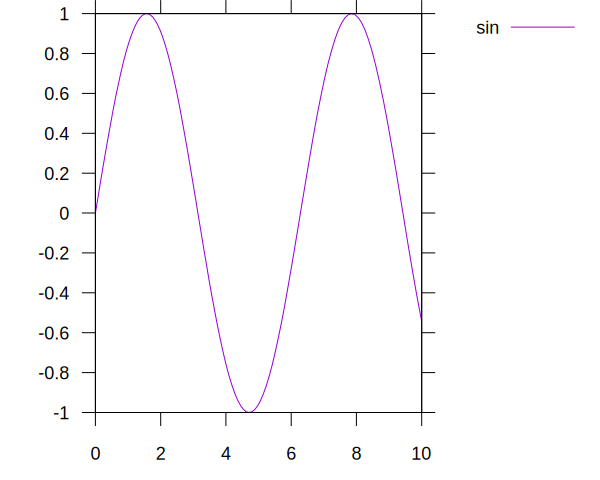
\includegraphics{plot}}%
    \gplfronttext
  \end{picture}%
\endgroup

\end{figure}


\end{document}